% JUMP TO LINE 60, 75
\documentclass{article}
\usepackage[letterpaper,portrait,top=0.4in, left=0.6in, right=0.6in, bottom=1in]{geometry}

\usepackage{amsmath, amsfonts, amsthm, amssymb}
\usepackage{graphicx, float}
\usepackage{suffix}
\usepackage{esdiff}
\usepackage{pdfpages}
\usepackage{multicol}
\usepackage{cancel}
\usepackage{mdframed}
\usepackage{mathtools}
\usepackage{tcolorbox}
\usepackage{hyperref}
\usepackage[per-mode=symbol]{siunitx}
\usepackage{setspace}
\usepackage{parskip}
\usepackage{titling}
\usepackage{mlmodern}

\newcommand{\alignedintertext}[1]{%
  \noalign{%
    \vtop{\hsize=\linewidth#1\par
    \expandafter}%
    \expandafter\prevdepth\the\prevdepth
  }%
}

\newcommand{\definition}[1]{\begin{tcolorbox}[colback=red!5!white,colframe=red!75!black,parbox=false] #1 \end{tcolorbox}}

\newcommand{\theorem}[2]{\begin{tcolorbox}[title={#1},colback=blue!5!white,colframe=blue!75!black,parbox=false] #2 \end{tcolorbox}}
\WithSuffix\newcommand\theorem*[1]{\begin{tcolorbox}[colback=blue!5!white,colframe=blue!75!black,parbox=false] #1 \end{tcolorbox}}

\newcommand{\example}[2]{\begin{tcolorbox}[title={Example: #1},colback=brown!5!white,colframe=brown!75!black,parbox=false] #2 \end{tcolorbox}}

\newcommand{\remark}[2]{\begin{tcolorbox}[title={#1},colback=black!5!white,colframe=black!75!black,parbox=false] #2 \end{tcolorbox}}
\WithSuffix\newcommand\remark*[1]{\begin{tcolorbox}[colback=black!5!white,colframe=black!75!black,parbox=false] #1 \end{tcolorbox}}

\newcommand*{\deriv}[1][x]{\ensuremath{\dfrac{\mathrm{d}}{\mathrm{d}#1}}}
\newcommand*{\floor}[1]{\ensuremath{\lfloor #1\rfloor}}

\title{\vspace*{-40pt}Notes on Multivariable Calculus}
\author{Jayden Li}
\date{\today}

\begin{document}
\setstretch{1.25}
\fontsize{11pt}{12pt}\selectfont
\setlength{\abovedisplayskip}{\abovedisplayskip/2}
\setlength{\belowdisplayskip}{\belowdisplayskip/2}
\setlength{\parindent}{0pt}
\setlength{\parskip}{2ex plus 0.5ex minus 0.2ex}
\maketitle

\section{Vectors}

\subsection{Basics}

Let $u,v$ be vectors in $\mathbb R^n$. They will have $n$ components, and let them be as follows, where $u_i,v_i\in\mathbb R$ (scalars):
\begin{align*}
	u&=(u_1,u_2,\ldots,u_n) \\
	v&=(v_1,v_2,\ldots,v_n)
\end{align*}
We can define the addition operation and the magnitude of each vector as:
\begin{align*}
	u+v&=(u_1+v_1,u_2+v_2,\ldots,u_n+v_n) \\
	\lVert u \rVert &=\sqrt{u_1^2+u_2^2+\ldots+u_n^2}=\sqrt{\sum_{i=1}^{n}u_i}
\end{align*}
Since scalar addition is commutative, so is vector addition. Also, the subtraction operation is defined as:
\begin{equation*}
    u-v=u+(-v)=(u_1-v_1,u_2-v_2,\ldots,u_n-v_n)
\end{equation*}
If we have two points $A$ and $B$, the vector $AB$ from $A$ to $B$ is given by $AB=B-A$. If we placed the tail of the vector at $A$, then the head will point to $B$.

Two vectors are parallel if and only if they are scalar multiples of each other; that is, there exists a scalar $a\in\mathbb R$ such that $u=av$.

\subsection{Polar Form}
For a vector $u\in\mathbb R^2$, we can write $u$ in polar form. Any vector can be specified with an angle from the $x$ axis and a magnitude. Let the angle from the $x$ axis be $\theta$ and the magnitude, the distance to the origin, be $r$. To convert from Cartesian to polar:
\begin{equation*}
    u=\begin{bmatrix}
		u_x \\ u_y
    \end{bmatrix}
	\implies \left\{\begin{aligned}
		\theta&=\arctan\left(\frac{u_y}{u_x}\right) \\
		r&=\lVert u \rVert =\sqrt{u_x^2+u_y^2}
	\end{aligned}\right.
\end{equation*}
To convert from polar to Cartesian:
\begin{equation*}
    u=\begin{bmatrix}
		r\cos\theta \\ r\sin\theta
    \end{bmatrix}
    =r\begin{bmatrix}
		\cos\theta \\ \sin\theta
    \end{bmatrix}
\end{equation*}
Note that since $\sin^2\theta+\cos^2\theta=1$ by the Pythagorean identity, the magnitude of $u$ is $r$.

\subsection{Unit Vectors}

A unit vector is a vector of magnitude $1$. For a vector $u\in\mathbb R^n$, a unit vector with the same direction is $u/\lVert u \rVert $.

\subsection{Dot Product}
For vectors $u=(u_1,\ldots,u_n)\in\mathbb R^n$ and $v=(v_1,\ldots,v_n)\in\mathbb R^n$, the cross product of the two vectors $u\cdot v$ is:
\begin{equation*}
    u\cdot v=u_1v_1+u_2v_2+\ldots+u_nv_n=\sum_{i=1}^{n}u_iv_i
\end{equation*}
Since scalar multiplication is commutative, so is the dot product: $u\cdot v=v\cdot u$.

Alternatively, let $\theta$ be the angle between vectors $u$ and $v$. Then:
\begin{equation*}
    u\cdot v=\lVert u \rVert \lVert v \rVert\cos\theta
\end{equation*}

\subsection{Orthogonality}

Two vectors $u$ and $v$ are orthogonal if and only if $u\cdot v=0$.

\subsection{Standard Bases}

The standard basis vectors are as follows:
\begin{align*}
	\hat i &= (1,0,0) \\
	\hat j &= (0,1,0) \\
	\hat k &= (0,0,1)
\end{align*}
These vectors span the $\mathbb R^3$ space.

\subsection{Angle Between Vectors}

We can calculate the angle between vectors $u,v\in\mathbb R^n$ using the cross product:
\begin{equation*}
    u\cdot v=\lVert u \rVert \lVert v \rVert \cos\theta
	\implies \cos\theta=\frac{u\cdot v}{\lVert u \rVert \lVert v \rVert }
\end{equation*}

\subsection{Cross Product}
The cross product only exists between vectors in three dimensions. Let $u=(u_x,u_y,u_z)\in\mathbb R^3$ and $v=(v_x,v_y,v_z)\in\mathbb R^3$. The cross product $u\times v$ has the following properties:
\begin{itemize}
	\item $u\times v$ is a vector in $\mathbb R^3$.
	\item $u\times v$ is orthogonal to both $u$ and $v$. If $u$ and $v$ are linearly independent and span a plane, $u\times v$ is orthogonal to that plane as well.
	\item $u\times v=0$ if and only if $u$ and $v$ are parallel/linearly dependent.
	\item The magnitude of $u\times v$ equals the area of the parallelogram formed by $u$ and $v$: $\lVert u\times v \rVert =\lVert u \rVert \lVert v \rVert \sin\theta$
\end{itemize}
The formula for $u\times v$ can be written concisely with a determinant, and expanding by cofactors:
\begin{equation*}
    u\times v 
	=\begin{vmatrix}
		\hat i & \hat j & \hat k \\
		u_x & u_y & u_z \\
		v_x & v_y & v_z \\
	\end{vmatrix} \\
	=\hat i \begin{vmatrix}
		u_y & u_z \\
		v_y & v_z
	\end{vmatrix}
	-\hat j \begin{vmatrix}
		u_x & u_z \\
		v_x & v_z
	\end{vmatrix}
	+\hat k \begin{vmatrix}
		u_x & u_y \\
		v_x & v_y
	\end{vmatrix}
\end{equation*}
The operation has the following properties:
\begin{itemize}
	\item Anticommutativity: $u\times v=-(v\times u)$
	\item Distributive over addition: $(u+v)\times w=u\times w+v\times w$ and $u\times(v+w)=u\times v+u\times w$.
	\item Multiplication by a scalar: $(cu)\times v=c(u\times v)=u\times(cv)$ where $c\in\mathbb R$.
\end{itemize}

The scalar triple product is the determinant of the square matrix with those vectors as its rows (or columns):
\begin{equation*}
	u\cdot(v\times w)
	=(v\times w)\cdot u
	=\begin{vmatrix}
		u_x & u_y & u_z \\
		v_x & v_y & v_z \\
		w_x & w_y & w_z \\
	\end{vmatrix}
\end{equation*}
From the determinant, it follows that the scalar triple product of $u,v,w$ is the volume of the parallelepiped with $u,v,w$ as its edges.

\subsection{Projection}

The orthogonal projection of $u$ onto $v$, written $\mathrm{proj}_v u$, is the vector parallel to $v$ such that the error between the projection and $u$ is minimized.

Let $p$ be the orthogonal projection $\mathrm{proj}_v u$. The error of the project is $e=u-p$. The error is minimized when $e$ is orthogonal to $v$. The formula for orthogonal projection is:
\begin{equation*}
	\mathrm{proj}_vu
	=\frac{u\cdot v}{v\cdot v}v
	=\frac{u\cdot v}{\lVert v \rVert ^2}v
\end{equation*}
The proof is left as an exercise to the reader.

\section{Lines}

A line in 3D space can be represented in three ways. In each subsection below, we specify a line passing through $(x_0,y_0,z_0)$ with slopes $a,b,c$.

\subsection{Parametric}

This parametric system with parameter $t$ describes the line we want:
\begin{equation*}
	\left\{\begin{aligned}
		x(t)&=at+x_0 \\
		y(t)&=bt+y_0 \\
		z(t)&=ct+z_0 \\
	\end{aligned}\right.
\end{equation*}

\subsection{Vector}

A vector valued function $f:\mathbb R\to \mathbb R^n$. It takes a scalar and returns a vector: $f(t)\in\mathbb R^n, t\in\mathbb R$.

From the parametric equation of a line, we notice that for parameter $t$, this point lies on the line. We can define a vector valued function $r$ with parameter $t$. This is the vector equation for a line.
\begin{equation*}
    r(t)
	=\begin{bmatrix}
		x \\ y \\ z
    \end{bmatrix}
	=\begin{bmatrix}
		at+x_0 \\
		bt+y_0 \\
		ct+z_0
	\end{bmatrix}
\end{equation*}

\subsection{Symmetric}

Recall the parametric system for a line. We solve for the parameter $t$ in terms of $x,y,z$ values:
\begin{equation*}
	\left\{\begin{aligned}
		x(t)&=at+x_0 \\
		y(t)&=bt+y_0 \\
		z(t)&=ct+z_0 \\
	\end{aligned}\right.
	\implies
	\left\{\begin{aligned}
		t&=\frac{x-x_0}{a} \\
		t&=\frac{y-y_0}{b} \\
		t&=\frac{z-z_0}{c} \\
	\end{aligned}\right.
\end{equation*}
For each equation in the above system, the parameter $t$ must be equal, yielding the symmetric equation of a line:
\begin{equation*}
    \frac{x-x_0}{a}=\frac{y-y_0}{b}=\frac{z-z_0}{c}
\end{equation*}

\subsection{Finding Intersection}
Suppose we have two lines with the following parametric equations:
\begin{equation*}
	\left\{\begin{aligned}
		x_1(t_1)&=a_1t_1+x_{10} \\
		y_1(t_1)&=b_1t_1+y_{10} \\
		z_1(t_1)&=c_1t_1+z_{10} \\
	\end{aligned}\right.
	\qquad
	\left\{\begin{aligned}
		x_2(t_2)&=a_2t_2+x_{20} \\
		y_2(t_2)&=b_2t_2+y_{20} \\
		z_2(t_2)&=c_2t_2+z_{20} \\
	\end{aligned}\right.
\end{equation*}
These two lines intersect exactly where $(x_1,y_1,z_1)=(x_2,y_2,z_2)$.
\begin{equation*}
	\left\{\begin{aligned}
		a_1t_1+x_{10}&=a_2t_2+x_{20} \\
		b_1t_1+y_{10}&=b_2t_2+y_{20} \\
		c_1t_1+z_{10}&=c_2t_2+z_{20} \\
	\end{aligned}\right.
\end{equation*}
We know the value of $a,b,c,x_0,y_0,z_0$ for both equations. There are two variables to solve: $t_1$ and $t_2$. But this is an overdetermined system, with three linear equations for two variables, so there is only a solution (and intersection) if these equations are not independent. If there is, then we can use $t_1$ and $t_2$ to find the point (or infinity points) of intersection.

\section{Planes}

The equation of a plane in 3D passing through $(x_0,y_0,z_0)$ is:
\begin{align*}
	a(x-x_0)+b(y-y_0)+c(z-z_0)&=0 \\
	\begin{bmatrix}
		x-x_0 \\
		y-y_0 \\
		z-z_0 \\
	\end{bmatrix}
	\cdot \begin{bmatrix}
		a \\ b \\ c
	\end{bmatrix}
	&=0
\end{align*}
Alternative, expanding the first equation, there exists a scalar value $d$ such that the plane is described by:
\begin{equation*}
	ax+by+cz+d=0
\end{equation*}
Subtracting by $x_0,y_0,z_0$ shifts the plane. The plane parallel to the original plane, but which passes through the origin, is given by $(x,y,z)\cdot(a,b,c)=0$. Which means that for all points on the plane, $(a,b,c)$ is orthogonal to it. Hence $n=(a,b,c)$ is orthogonal to the plane.

\subsection{Dihedral Angle}

The dihedral angle is the angle formed between two planes. It equals the angle formed between the normal vectors of each plane, which can be found using the dot product.

\subsection{Angle between Vector and Plane}

Let $v$ be the vector. Find the normal vector to the plane $n$, and find the angle $\theta$ between the vector and $n$. The angle between the plane and $v$ is $90^\circ-\theta=\pi/2-\theta$.

\subsection{Finding Intersection}

Two planes intersect if and only if the vectors normal to the plane point in different direction and are not parallel.
\begin{align*}
    a_1x+b_1y+c_1z+d_1&=0 \\
    a_2x+b_2y+c_2z+d_2&=0
\end{align*}
A point on the intersection of these two planes satisfy both equations. From here, set any variables ($x,y,z$) to a parameter $t$ and substitute. Then use elimination to solve for the two remaining variables in terms of $t$ (DO NOT ELIMINATE $t$). Now we have a parametric system describing the line of intersection.

\section{Cylinders and Quadric Surfaces}

\begin{center}
	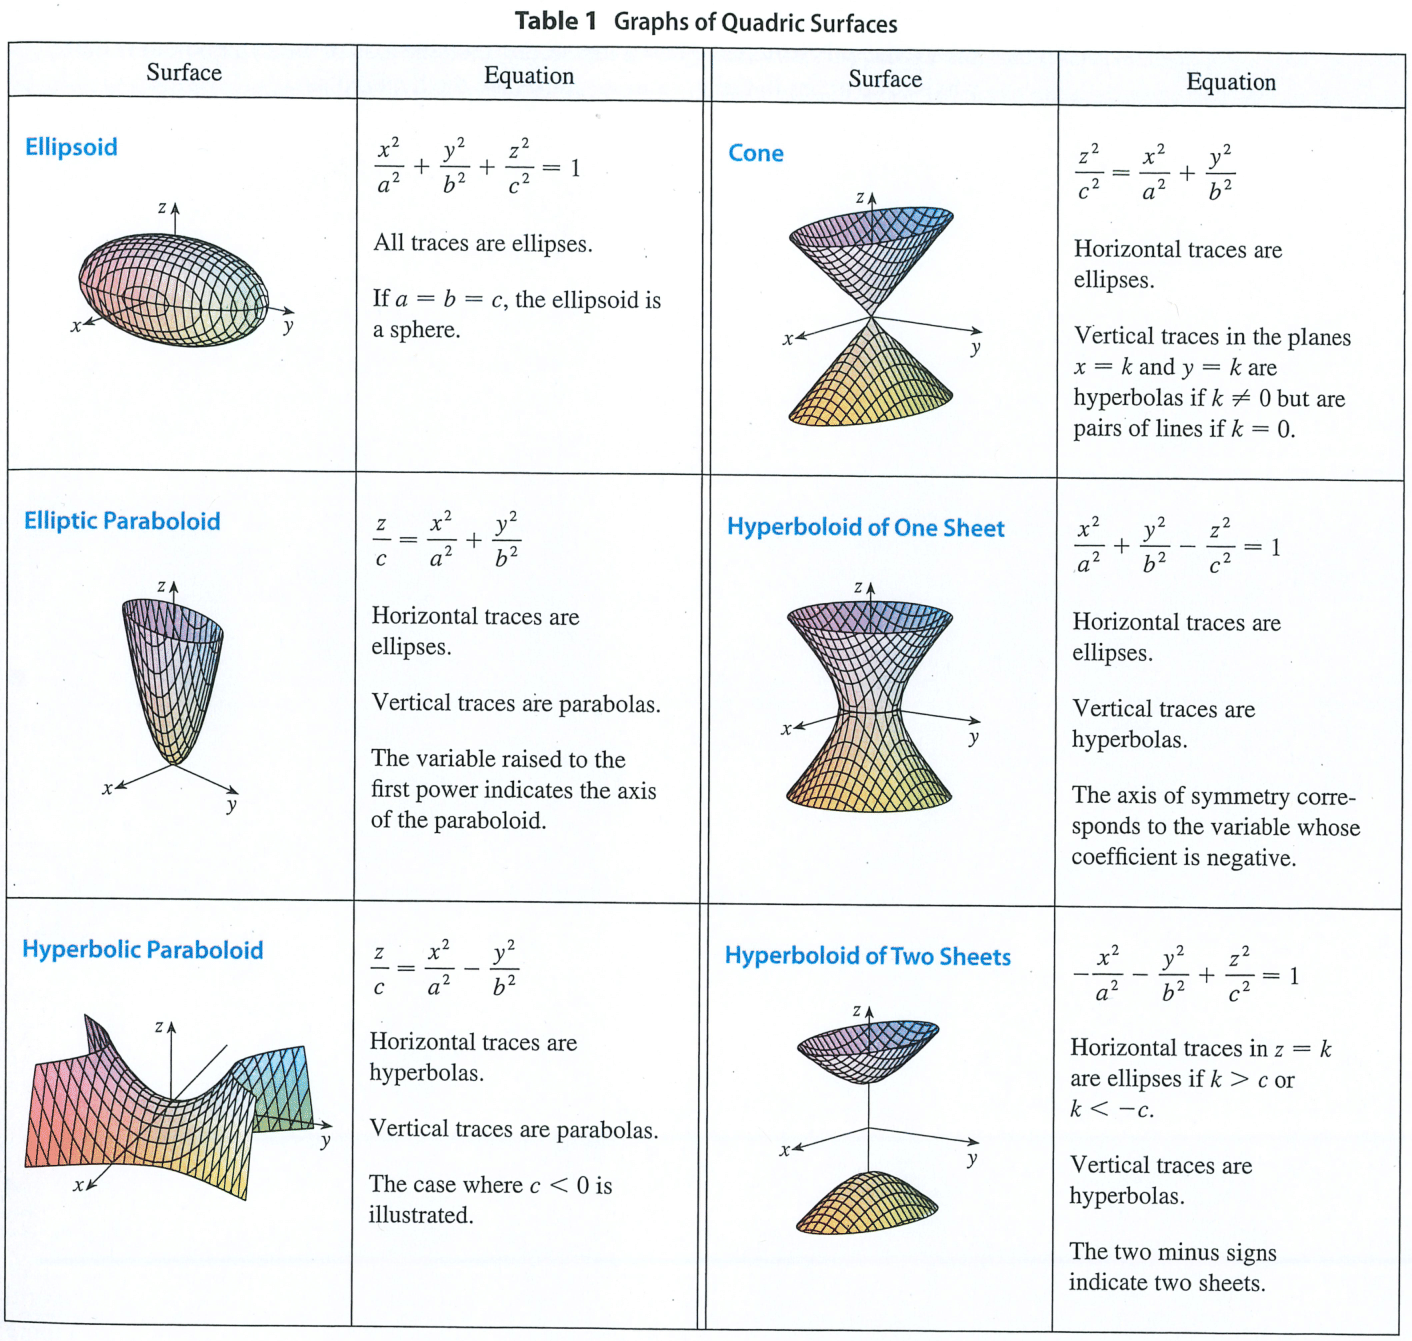
\includegraphics[width=\linewidth]{quadric.png}
\end{center}

\subsection{Trace}

The intersection of a quadric surface with a plane normal to a standard basis vector is a trace. We can use the trace produced by a equation in each direction to determine which quadric surface the equation is.

\subsection{Cylinders}

A cylinder is a surface that consists of all lines that are parallel to a given line, and which passes through a plane curve. For example, the surface given by $y=x^2$ is a cylinder because the $z$ component of each point can be anything, hence every line is parallel to $\hat k$.


\end{document}
